\documentclass{isddmaster}
\usepackage[skip=3pt plus1pt]{parskip}
\setlength{\textfloatsep}{12pt plus 2pt minus 4pt}
\setlength{\intextsep}{10pt plus 2pt minus 4pt}
\usepackage{titlesec}
\usepackage{floatrow}
\usepackage{lipsum}
\titlespacing*{\subsection}{0pt}{12pt}{4pt}
\onehalfspacing

\begin{document}
	
	\checkyears
	
	\vspace*{5mm}
	
	\setkeys{Gin}{draft=false}
	
	\selectlanguage{french}   
	
	\def\title{Projet de Criblage Virtuel \\[5mm] \normalsize \textit{UE "Chemoinformatics tools for biological therapeutics"}}


	
	\def\spe{Modélisation des macromolécules} 
	% \def\scientificmanager{L. Regad \& M. Baillif}
	\def\author{Anna Perova}
	\def\studentnumber{22519413}
	\def\shorttitle{Rapport Criblage}
	\def\mydate{\today}
	
	\pagenumbering{gobble}
	\Entete
	\medskip
	\begin{abstract}
		{\small \textbf{Résumé:} 
		
		\textbf{Mots clés:} }
	\end{abstract}
	
	\vfill
	
	%\newpage
	%\tableofcontents
	\newpage
	
	\pagenumbering{arabic}
	\setcounter{page}{1}
	\section{Introduction}
	\textbf{HMG-CoA Reductase} ou 3-hydroxy-3-methyl-glutaryl-coenzyme A reductase ou HMGCR est une enzyme qui de la voie métabolique de production du cholestérol ainsi que d'autres isoprénoïdes via la voie de biosynthèse qui catalyse la transformation du HMG-CoA en L-mévalonate.
	Les inhibiteurs du HMRG, son surtout utilisées pour traiter la dyslipidémie qui se traduisent par une concentration anormalement élevée ou diminuée de lipides dans le sang. Les taux abnormales du cholésterol sont courrament au cause de maladies cardiovasulaires. 
	Plus connus sous le nom des statins, les inhibiteurs du HMGCR sont étudiées depuis les années 70s \cite{endoML236AML236BML236C1976b,endoCompetitiveInhibition3hydroxy3methylglutaryl1976} et vers 90s la benefice du traitement chez les coronariens a était démontré \cite{RandomisedTrialCholesterol}.
	Leur action repose sur l'occupation du site actif de l'enzyme à la place du substrat [3], [4]. Malgré leur efficacité, utilisation des statines à long-terme entraînent des effets secondaires comme faiblesse musculaire, douleurs nerveuses, surcharge hépatique et fatigue. De plus, certains patients ont des predispositions génétiques qui causent les intolerances pour les statins, d'ou vient interet pour la recherche de structures chimiques alternatives.
	Developpement des pipelines et modéles predictives efficaces pour le criblage virtuel, pourrait accélérer le processus du developement pharmaceutique.

	L'objectif de ce projet était d'établir un pipeline pour une procedure de criblage virtuel, contre la cible bien étudié et validée pharmacologiquement.
	Cela nous permet de developper un méthode de criblage virtuel qu'on peut tester avec les données bien étiquetée avant de l'appliquer pour le screening des structures dont on ne connait pas l'activité.
	Ici, on décrit le processus d'extraction du nombre maximal de composés actifs parmi les composés les mieux classés d'un ensemble de 151 composés actifs / 8324 composés inactifs, en utilisant des approches basées sur les ligands, sur la structure et sur le consensus, en appliquant une modéle de Regression Logistique et Random Forest.
	
	
	
	\section{Préparation des données}
	Les fichiers .smi avec les numeros d'identification CHEMBL et la structure en format SMILES ont été fournis pour ce projet \footnote{\href{https://owncloud.rpbs.univ-paris-diderot.fr/owncloud/index.php/s/J3z2UQGxRhSr5YY}{Lien pour les donées}}. Il contient 151 composées actifs et 8 324 composés inactifs.
	Le traitement de données et l'analyse a été effectué dans le notebook Jupyter en Python \footnote{\href{https://github.com/annhater/My-Vault}{Donées pour l'ensemble de projet sur GitHub}}.
	Depuis ces données là, on a réalisé une verification d'activité de ces composées avec la métrique IC50 (Concentration inhibitrice à $50\% \geq 6.5$ nM). Puis, on a confirmé l'absence de duplicats dans le dataset, et preparé les structures SMILES pour traitement à suivre en supprimant les sels avec le package \lstinline{RDKit}.
	20 structures choisies aléatoirement ont été retenus comme les structures actives de référence pour calculer le taux de similarité par la suite (Fig.\ref{ref_set}). Ainsi, pour l'étape de ligand-based screening, on a 280 molécules actives et 8324 molécules inactives.


	\section{Ligand-based screening}
	
	Les empreintes de Morgan (2048 bits, rayon 2) et MACCS (167 bits) ont été calculées sur l'ensemble des molécules.
	Avec les empreintes calculées, on a pu obtenir les taux de similarité (Tanimoto et Dice).
	\begin{wrapfigure}[9]{r}{0.45\textwidth}
		\vspace{-20mm}
		\begin{center}
			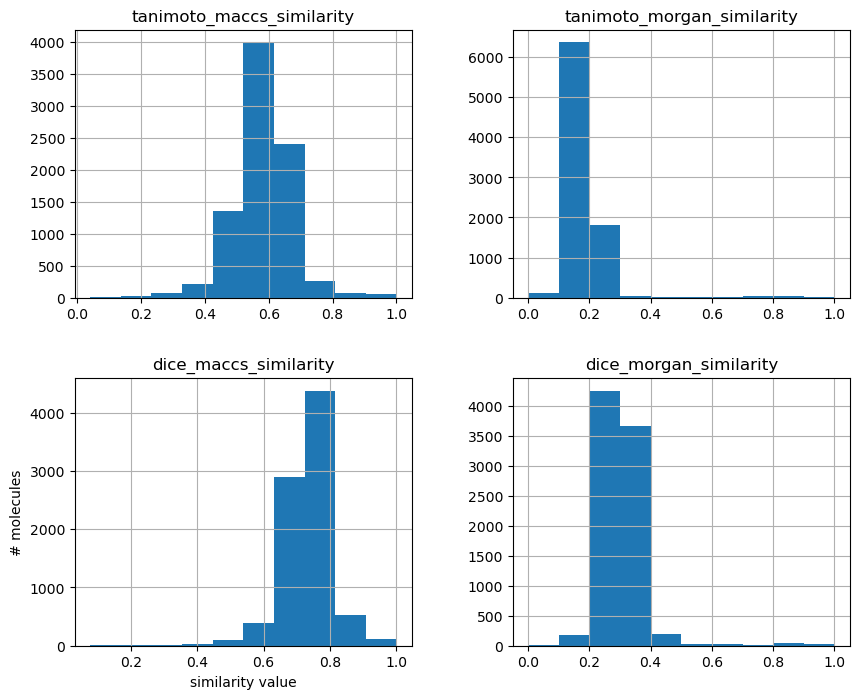
\includegraphics[width=\textwidth]{Figures/sim_hist.png}
			\caption{Dataset de molécules actives choisies comme référence pour Ligand-based screening.}
		\label{fig:hist}
		\end{center}
	\end{wrapfigure}
	En analysant les distributions de ces scores, on a pu confirmer que les clés de MACCS resultent en taux de similarité moins élevées – logique vu la haute sensitivité de son algorithme, qui capture l'environnement atomique plus detaillés.
	De plus, on à observé que le taux de similarité de Dice a une tendance de donner des valeurs plus élevées, du a son mode de calcul (plus de poids à l'intersection). Vue qu'on ne veut pas trop priviligier les similarités entre les molécules actives et inactives ainsi que capter l'environnement chimique le plus précis possible, par la suit on privilège le score \lstinline{tanimoto_morgan_similarity}.     
	



	\begin{wrapfigure}[15]{r}{0.45\textwidth}
		\begin{center}
			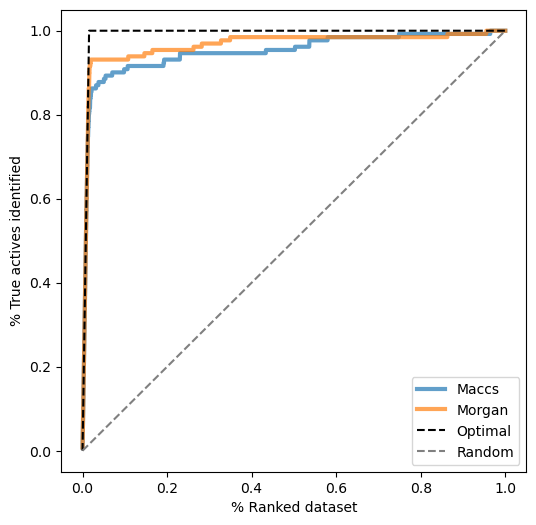
\includegraphics[width=\linewidth]{Figures/roc_ligand.png}
			\label{fig:roc-ligand}
		\end{center}
		\caption{Courbe d'enrichissement pour les deux métriques: score de Tanimoto avec les empreintes de Morgan (orange, AUC = $93.1\%$) ou de MACCS (bleu, AUC = $87.8\%$)}
	\end{wrapfigure}
	Par la suite, afin d'évaluer et valider les résultats du criblage virtuel basé sur les ligands, on a construit les courbes d'enrichisemment. Ils affichent la proportion de molécules actives détectées dans les top x\% du classement. C'est-à-dire la proportion de molécules les mieux classées dans l'ensemble des données par rapport à la proportion de molécules actives vraies dans l'ensemble des données.
	Les valeurs pour EF5\% (enrichment factor pour les top 5\%) évalué sur la bibliothèque complète, demontrent que la méthode de criblage virtuel qui utilisé les empreintes de Morgan identifie avec succès une proportion plus élevée de molécules réellement actives dès le début de la liste classée, comparativement à une sélection aléatoire.
	\textit{Conclusion for Ligand-based}
\vspace{15mm}
	\section{Structure-based screening (docking)}
	\begin{wrapfigure}[15]{r}{0.45\textwidth}
		\vspace{22mm}
		\begin{center}
			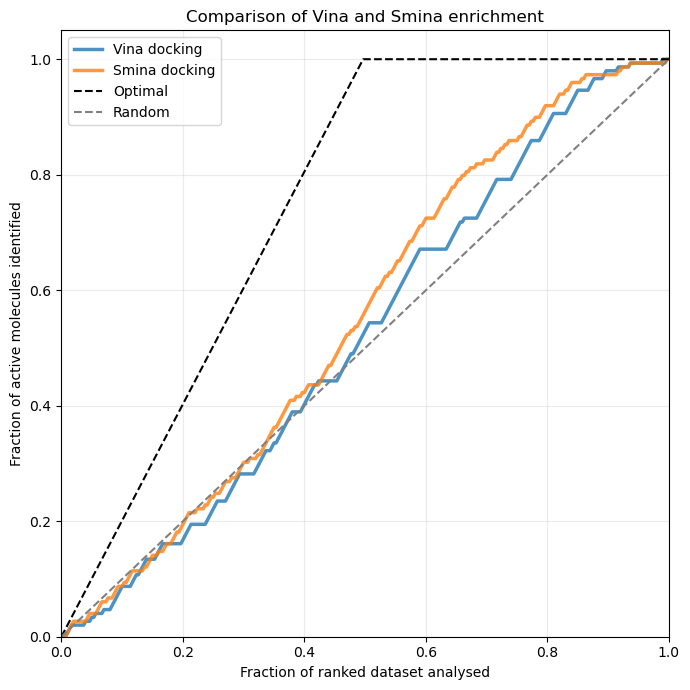
\includegraphics[width=\linewidth]{Figures/vina-smina.png}
			\label{fig:vina-smina}
		\end{center}
		\caption{Courbe d'enrichissement pour les deux outils de docking: Smina (orange, AUC =$40\%$) ou Vina (bleu, AUC = $\%$)}
	\end{wrapfigure}
	L'étude de la structure des ligand est une bonne piste pour analyse pré-liminaire, néanmoins, il est aussi important de comprendre le façon dans lequel le ligand interagit avec le cible/récepteur. Pour cela, on applique les méthodes d'amarrage moléculaire ou docking.
	La structure utilisé pour l'ammarage est celui de 3CCW sur le PDB \footnote{\href{https://www.rcsb.org/structure/3CCW}{Entrée web sur PDB}}, produit de co-cristalisation de HMGCR avec 4HI (molécule ressemblante au statins \footnote{\href{https://www.ebi.ac.uk/chembl/explore/compound/CHEMBL488636}{Entrée CHEMBL}}) obtenu avec diffraction au rayon X avec résolution de 2.1\AA.
	Afin de préparer la structure pour l'ammarage, on à éliminé l'eau, assigné les charges, converti le fichier du type \lstinline{.mol2} à \lstinline{.pdbqt} avec l'outil OpenBabel \footnote{\href{https://openbabel.org/index.html}{Site web de OpenBabel}}.
	Le centre de la boite de docking ont était déteriminé à partir du centre du ligand 4HI dans la structure d'origine (x: 4.76321, y: 31.71096, z: 6.64880) et taille de la boite $30\times30\times30 \AA$.


	\begin{figure}[h!]
		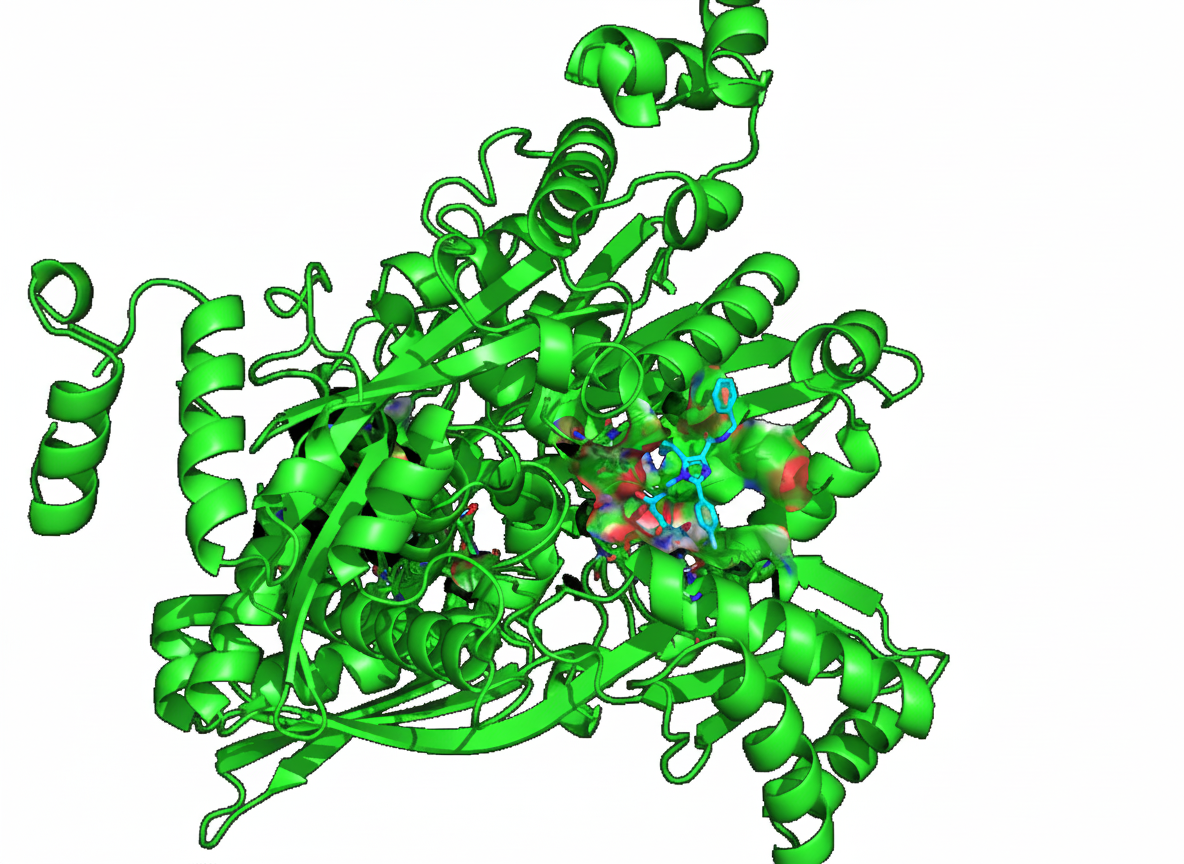
\includegraphics[width=0.6\textwidth]{Figures/3CCW.png}
		\caption{Represenation 3D de HMGCR (vert) avec ligand 4HI (cyan) dans le poche d'interaction en PyMol. PDB: 3CCW}
		\label{fig:ref_set}
	\end{figure}

	Pour les 151 ligands actives et 151 inactives (choisis aléatoiremet) une structure \lstinline{.pdbqt} à était générée avec OpenBabel (seulement 149 actives rétenus pour docking car on n'a pas pu générer des structures 3D pour CHEMBL3704922 et CHEMBL3704923). Ce choix de retenir seulement 151 molécules inactives de 8 324 composées d'origine est explique surtout par les contraintes de temps (docking de ce volume prendra $\approx 5$ jours). La fraction de dataset inactive pour docking nous permet non seulement d'efferctuer deux types de docking afin de le comparer leur résultats, mais aussi resulte en dataset equilibré avec la portion des molécules actives (une desequilibre peut produire des biais dans les modéles d'apprentissage d'après).  
	Deux logiciels de docking ont été utilisées : AutoDock Vina et Smina (une version dérivée d'AutoDock Vina offrant des fonctionnalités améliorées pour le développement de fonctions de score et la minimisation d'énergie haute performance).
	Après le docking, les scores d'energie potentielle de la premiere pose (la plus favorable énergitiquement) a été extrait ainsi que les données d'enrichissement.
	Sur les courbes d'enrichissement on observe que Smina a une meilleur perfomance par rapport à AutoDock Vina, par contre les deux outils de docking ont peu de difference contre la courbe d'enrichissement dite aléatoire (le score obtenu en sélectionnant des composés de manière totalement aléatoire, $50/50$).
	Ceci est confirmé globalement par la littrature, qui indique que Vina et son d'amarrage brute est souvent moins performante qu'une combinaison d'informations \cite{Confidence}.

	Ainsi, par la suite on essay de mettre en place une modéle predictive (Regression Logistique) qui prends en compte les resultats consensus du ligand et structure-based screening. 
	
	\section{Méthode consensus (Apprentissage Automatique)}

	Pour entrainer des modéles de Regression Linéaire et de Random Forest on a pris deux descripteurs :  score de similarité (Tanimoto et Morgan) + score d'amarrage (Smina). Lors du developpement de la modéle, on s'est rendu compte une sur-apprentissage de la modéle (indiqué par les métriques le recall et accuracy près de 1).
	Afin d'éviter ce genre de sur-apprentissage, on veut éviter que les des structures trop similaires ne sont pas reparties entre les sets d'apprentissage et d'entrainement, mais restent dans l'un de deux sets.
	Pour cela, on a appliqué l'approche de Bermis et Murko introduit en 1996 et qui fait partie du RDKit \cite{bemisPropertiesKnownDrugs1996,huLessonsLearnedMolecular2011}. 

	En analysant les performances de deux modéles consensus\ref{all}, on note que RF est bien plus performant que la modéle LogReg. C'est une résultat attendu, vue que RF permet gérer les parametres non-linéaires ainsi que multicolinéarité présente entre les deux paramétres.
	Néanmoins, en comparant avec les autres tests réalisées, on observe que lorsque on analyse ce subset de ligands sans l'apprentissage automatique aves les données issus de docking, le performance se prouve plus optimale. Cela peut indiquer que pour ce subset, les résultats de docking apporte une complexité additionelle, qui diminue le performance.
	Cela étant dit, on ne peut pas dire que ce méthode sera autant performant avec un autre subset ou bien avec les données completement nouvelles/non-etiquettées. Il est preferable de laisser le modéle consensus qui apporte l'information de deux cotés – de ligands et de récepteurs.
	

% RF accuracy:  0.92
% RF precision: 0.93
% RF recall:    0.87
% RF F1:        0.90
% RF AUC:       0.06
    \begin{wrapfigure}{r}{0.45\textwidth}
		% \vspace{-22mm}
		\begin{center}
			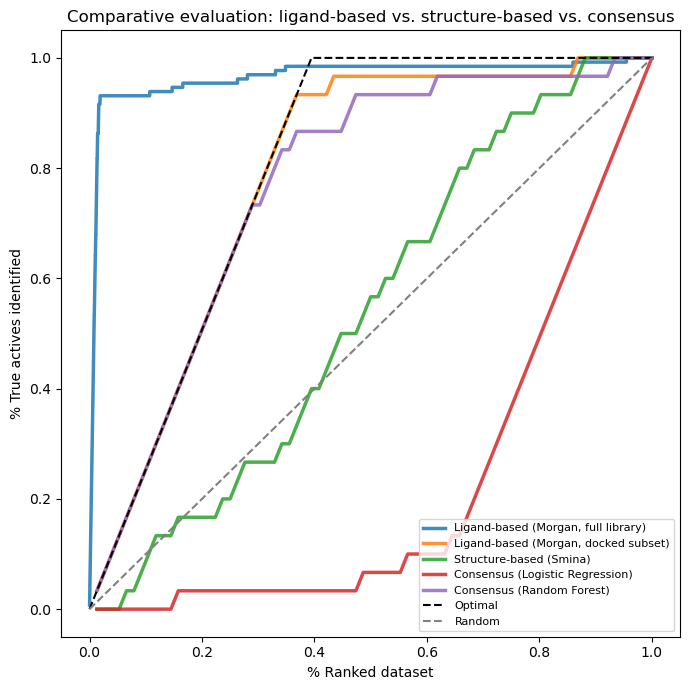
\includegraphics[width=\linewidth]{Figures/comparative_evaluation.png}
			\label{fig:all}
		\end{center}
		\caption{Placeholder}
	\end{wrapfigure}
	
\section{Discussion et Conclusion}
	Ce projet de criblage virtuel nous a permis de . Le méthode basé sur les ligands est capable d'analyser la bibliothèque complète avec haut niveau de performance. Les résultats basés sur la structure/le consensus sont limités à un sous-échantillon représentatif en raison du coût de l'amarrage moléculaire, pourtant ces données peuvent apporter des caracteristiques indispensables qui peuvent se rendre utiles lors d'application de cette modéle sur le set réel et non-étiaqutée.
	Malgré le presence des structurellement proches des composés actifs, mais réellement inactifs expérimentalement (decoys), avec notre méthode on a pu distinguer les molecules actives (Top 10 molécules de Tanimoto-Morgan similarité sont exclusivement actives). 
	En perspective il serait interessant de tester ce protocole contre un benchmark public externe (DUD-E/DEKOIS), afin de confirmer l'efficacité sur les données nouvelles.
	\begin{figure}[h!]
		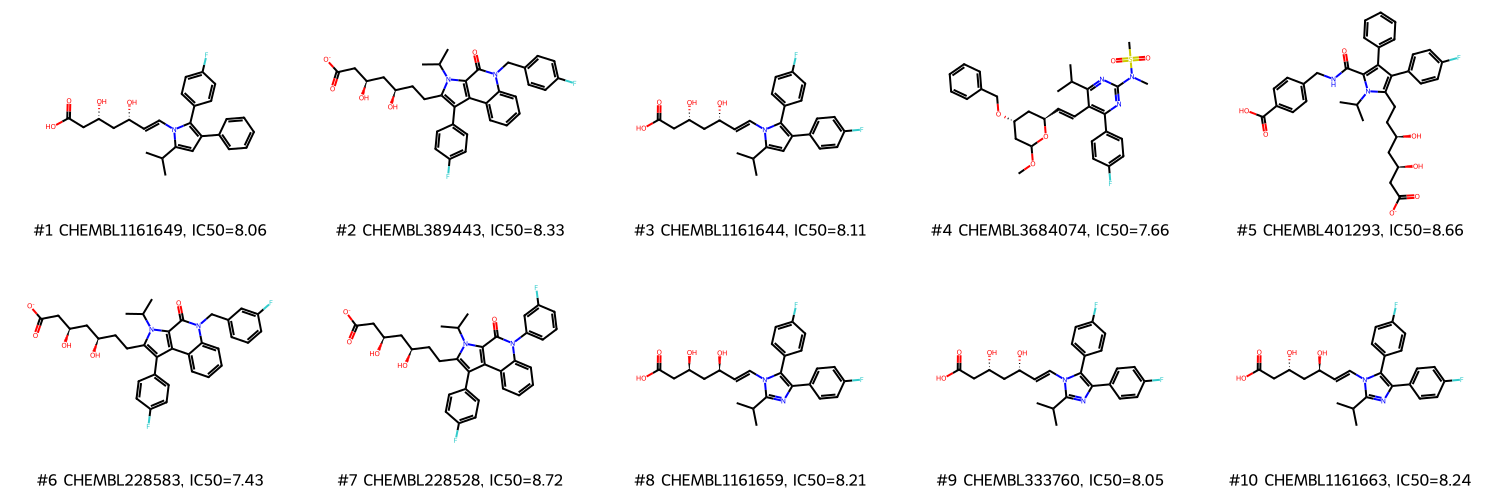
\includegraphics[width=\textwidth]{Figures/top-10.png}
		\caption{Les top dix molécules les scores de similarité les plus élévées contre les actives de référence. Toutes ces molécules font partie de dataset des molécules actives d'origine.}
		\label{fig:top-10}
	\end{figure}
	\newpage
	\addcontentsline{toc}{section}{Références}
	\bibliographystyle{unsrt} 
	\bibliography{masterBib} 
	\newpage
	\section{Annexe}

	\cleardoublepage
	
\end{document}

		\begin{wraptable}[9]{r}{0.8\textwidth}
		\vspace{-10pt}
			\centering
		\begin{tabular}{@{}lll@{}}
			\toprule
			\textbf{Condition} & \textbf{Nom}  & \textbf{Tps de sim (ns)}  \\ \midrule
			Déprototoné (DP)   & V11          & 1 000       \\
			Déprototoné (DP)   & V12          & 1 000       \\
			Déprototoné (DP)   & V1           & 1 000       \\
			Monoprotoné (MP)   & V7           & 1 000               
		\end{tabular}
		\caption{Tableau récapitulant les 6 simulations étudiées et ses conditions}
		\label{tab:simulations}
	\end{wraptable}     
	\end{figure}
	

	
	\begin{figure}[h!]
		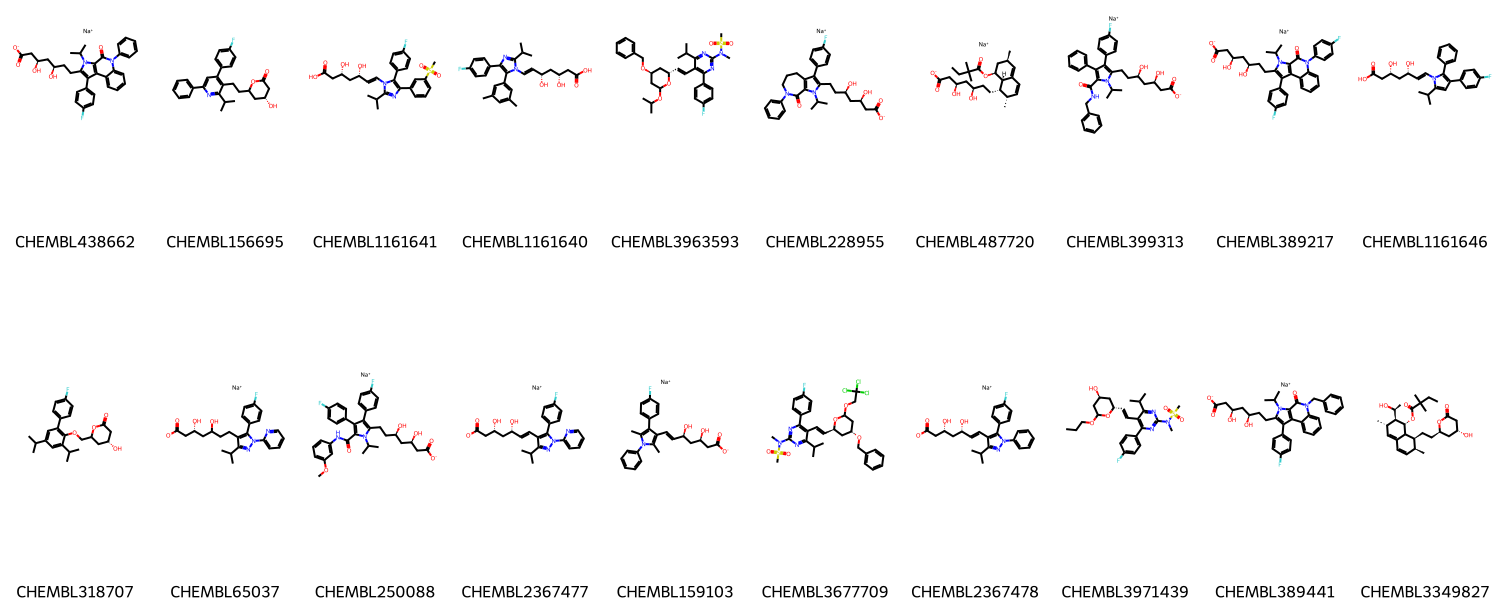
\includegraphics[width=\textwidth]{Figures/ref_set.png}
		\caption{Dataset de molécules actives choisies comme référence pour Ligand-based screening.}
		\label{fig:ref_set}
	\end{figure}
